%%%%%%%%%%%%%%%%%%%%%%%%%%%%%%%%%%%%%%%%%%%%%%%%%%%%%%%%%%%%%%%%%%%%%%%%%%%%%%%%
\documentclass[twocolumn]{revtex4}

%%%%%%%%%%%%%%%%%%%%%%%%%%%%%%%%%%%%%%%%%%%%%%%%%%%%%%%%%%%%%%%%%%%%%%%%%%%%%%%%
% Note that comments begin with a "%" and are not turned into text in the .pdf
% document.
%%%%%%%%%%%%%%%%%%%%%%%%%%%%%%%%%%%%%%%%%%%%%%%%%%%%%%%%%%%%%%%%%%%%%%%%%%%%%%%%

%%%%%%%%%%%%%%%%%%%%%%%%%%%%%%%%%%%%%%%%%%%%%%%%%%%%%%%%%%%%%%%%%%%%%%%%%%%%%%%%
% Include some extra packages.
%%%%%%%%%%%%%%%%%%%%%%%%%%%%%%%%%%%%%%%%%%%%%%%%%%%%%%%%%%%%%%%%%%%%%%%%%%%%%%%%
\usepackage[]{graphicx}
%%%%%%%%%%%%%%%%%%%%%%%%%%%%%%%%%%%%%%%%%%%%%%%%%%%%%%%%%%%%%%%%%%%%%%%%%%%%%%%%

%%%%%%%%%%%%%%%%%%%%%%%%%%%%%%%%%%%%%%%%%%%%%%%%%%%%%%%%%%%%%%%%%%%%%%%%%%%%%%%%
\begin{document}

%%%%%%%%%%%%%%%%%%%%%%%%%%%%%%%%%%%%%%%%%%%%%%%%%%%%%%%%%%%%%%%%%%%%%%%%%%%%%%%%
\title{
Prediciting the Weather
}

\author{Mafuse ~Solomon}

\affiliation{Siena College, Loudonville, NY}

\date{\today}

\begin{abstract}
The main objective of this project was to predict the weather.  More specifically predicting the odds of it raining or not. So the first question was "suppose there is a 20 percent chance it will rain on any given day in a month. What are the odds that that rains on one and only one day in a month?"  The answer I got was 9170/1000000 or .9 percent.  The second question I answered was "Suppose there is a 10 percent chance that it will rain on any given day in a month. What are the odds that it rains at least 8 days (in any order) that month?" The asnwer I got was 7754/1000000 or .7 percent.
\end{abstract}

\maketitle
%%%%%%%%%%%%%%%%%%%%%%%%%%%%%%%%%%%%%%%%%%%%%%%%%%%%%%%%%%%%%%%%%%%%%%%%%%%%%%%%

%%%%%%%%%%%%%%%%%%%%%%%%%%%%%%%%%%%%%%%%%%%%%%%%%%%%%%%%%%%%%%%%%%%%%%%%%%%%%%%%
\section{Introduction}
%%%%%%%%%%%%%%%%%%%%%%%%%%%%%%%%%%%%%%%%%%%%%%%%%%%%%%%%%%%%%%%%%%%%%%%%%%%%%%%%
The overall goal of the project is to figure out the odds of it raining given the percentage chance for certain days.  You should do this using the monte carlo approach we did in class for the birthday problem.

%%%%%%%%%%%%%%%%%%%%%%%%%%%%%%%%%%%%%%%%%%%%%%%%%%%%%%%%%%%%%%%%%%%%%%%%%%%%%%%%
\section{Problem 1}
%%%%%%%%%%%%%%%%%%%%%%%%%%%%%%%%%%%%%%%%%%%%%%%%%%%%%%%%%%%%%%%%%%%%%%%%%%%%%%%%
I create a function chance rain. I then generate a random number and set the variable rainprb equal to 0 however if the random number is equal to or between 0 and .2 the rainprb = 1.  I then tell the fuction to return rainprb.  
I create another function month and in it I make an empty list called rain days.  I loop over variable i 30 times.  I call my function from earlier chance rain by setting it equal to rain.  Then i append the function to the empty list.  i set variable x to the sum of the list rain days.  Then i said if x is 1 return 1 if not return 0.
I create a variable months equal to 1000000 which how many times i loop the variable i over. i call the last function month by setting it equal to day rained i then append it to the empty list i created called rained.  I take the sum of rained and set equal to the variable x.
i then print x which is the number of days rained that occured over 1000000 months.  I divide it by 1000000 to get a decimal which leads me to getting the percentage .9 percent or .00917 in decimal form.
%%%%%%%%%%%%%%%%%%%%%%%%%%%%%%%%%%%%%%%%%%%%%%%%%%%%%%%%%%%%%%%%%%%%%%%%%%%%%%%%
\section{Problem 2}
%%%%%%%%%%%%%%%%%%%%%%%%%%%%%%%%%%%%%%%%%%%%%%%%%%%%%%%%%
%%%%%%%%%%%%%%%%%%%%%%%

Problem 2 was the same setup as problem except i had to change the percentage to 10percent  instead of 20percent and instead of the odds of it raining  one day it was the odds of it raining at least 8 days.
I create a function chance rain. I then generate a random number and set the variable rainprb equal to 0 however if the random number is equal to or between 0 and .1 the rainprb = 1.  I then tell the fuction to return rainprb.  
I create another function month and in it I make an empty list called rain days.  I loop over variable i 30 times.  I call my function from earlier chance rain by setting it equal to rain.  Then i append the function to the empty list.  i set variable x to the sum of the list rain days.  Then i said if x is greater than or equal to 8 return 1 if not return 0.
I create a variable months equal to 1000000 which how many times i loop the variable i over. i call the last function month by setting it equal to day rained i then append it to the empty list i created called rained.  I take the sum of rained and set equal to the variable x.
i then print x which is the number of days rained that occured over 1000000 months.  I divide it by 1000000 to get a decimal which leads me to getting the percentage .7 percent or .007754  in decimal form

%%%%%%%%%%%%%%%%%%%%%%%%%%%%%%%%%%%%%%%%%%%%%%%%%%%%%%%%%%
%%%%%%%%%%%%%%%%%%%%%%%
\section{Calculus}
%%%%%%%%%%%%%%%%%%%%%%%%%%%%%%%%%%%%%%%%%%%%%%%%%%%%%%%%%%
%%%%%%%%%%%%%%%%%%%%%%%
One class I'm taking this semester at Siena College is calculus.  It is taught by Proffessor Campchero.  He has taught us alot about the unit circle this semester.  Which will be shown in the figures section.
%%%%%%%%%%%%%%%%%%%%%%%%%%%%%%%%%%%%%%%%%%%%%%%%%%%%%%%%%%
%%%%%%%%%%%%%%%%%%%%%%%
\section{Figures}

\begin{figure}[h]
	\centering
	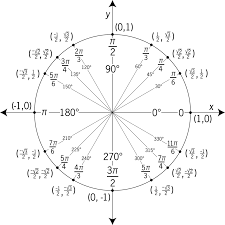
\includegraphics[width = 0.5\textwidth]{unitcircle.png}
	\caption{This is the Unit Circle! \label{Unit Circle}}


\end{figure}

Check out what I learned in calculus in Fig."\ref{Unit Circle}

%%%%%%%%%%%%%%%%%%%%%%%%%%%%%%%%%%%%%%%%%%%%%%%%%%%%%%%%%
%%%%%%%%%%%%%%%%%%%%%%%
\end{document}
%%%%%%%%%%%%%%%%%%%%%%%%%%%%%%%%%%%%%%%%%%%%%%%%%%%%%%%%%%%%%%%%%%%%%%%%%%%%%%%%
